\documentclass[12pt]{article}
\usepackage[utf8]{inputenc}
\usepackage{float}
\usepackage{amsmath}


\usepackage[hmargin=3cm,vmargin=6.0cm]{geometry}
%\topmargin=0cm
\topmargin=-2cm
\addtolength{\textheight}{6.5cm}
\addtolength{\textwidth}{2.0cm}
%\setlength{\leftmargin}{-5cm}
\setlength{\oddsidemargin}{0.0cm}
\setlength{\evensidemargin}{0.0cm}

%misc libraries goes here
\usepackage{tikz}
\usetikzlibrary{automata,positioning}

\begin{document}

\section*{Student Information } 
%Write your full name and id number between the colon and newline
%Put one empty space character after colon and before newline
Full Name :  Can Erdoğar \\
Id Number :  1942069 \\

% Write your answers below the section tags
\section*{Answer 1}

\subsection*{a.}
\begin{table}[H]
	\small
	\label{Q1-A}
	\begin{tabular}{|c|c|}	%% specify column number
	\hline
	Table 1 \\
	\hline 
	$r_1$ & $-0.d_{11}d_{12}d_{13}d_{14}...$ \\			%% rows distinguished with &
	$r_2$ & $-0.d_{21}d_{22}d_{23}d_{24}...$ \\
	$r_3$ & $-0.d_{31}d_{32}d_{33}d_{34}...$ \\
	$r_4$ & $-0.d_{41}d_{42}d_{43}d_{44}...$ \\
	. & . \\
	. & . \\
	\hline 

	\end{tabular}
\end{table}

Table 1 shows decimal representation of the numbers between 0 and -1. Then form a new number $r=0. d_1 d_2 d_3 ...$ and make $d_i= 9 - d_{ii}$.\\
However, this new number will differ from first number in the table with its first digit, second number with its second digit and so on. \\
This shows that r is not in the set and numbers between 0 and -1 cannot be listed, so it is uncountable. 

\subsection*{b.}
L is regular because it's finite as stated.That's why $L^{*}$ and $L^{+}$ will also be regular which makes D an empty set. \\

\section*{Answer 2}
a) \\
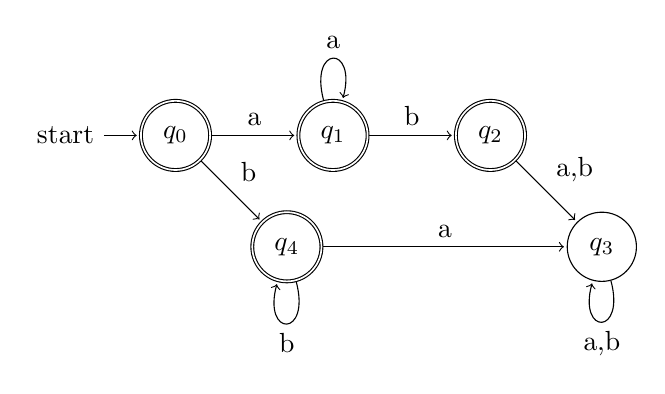
\begin{tikzpicture}[shorten >=1pt,node distance=2cm,on grid,auto]
\node[state ,initial,accepting] (q_0) {$q_0$};
\node[state,accepting] (q_1) [right=of q_0] {$q_1$}; 
\node[state,accepting] (q_2) [right=of q_1] {$q_2$};
\node[state] (q_3) [below right=of q_2] {$q_3$};
\node[state,accepting] (q_4) [below right=of q_0] {$q_4$};
 \path[->]
(q_0) edge node {a} (q_1)
(q_1) edge node {b} (q_2)
(q_1) edge [loop above] node {a} ()
(q_2) edge node {a,b} (q_3)
(q_0) edge node {b} (q_4)
(q_4) edge node {a} (q_3)
(q_4) edge [loop below] node {b} ()
(q_3) edge [loop below] node {a,b} ();
\end{tikzpicture}

b) \\
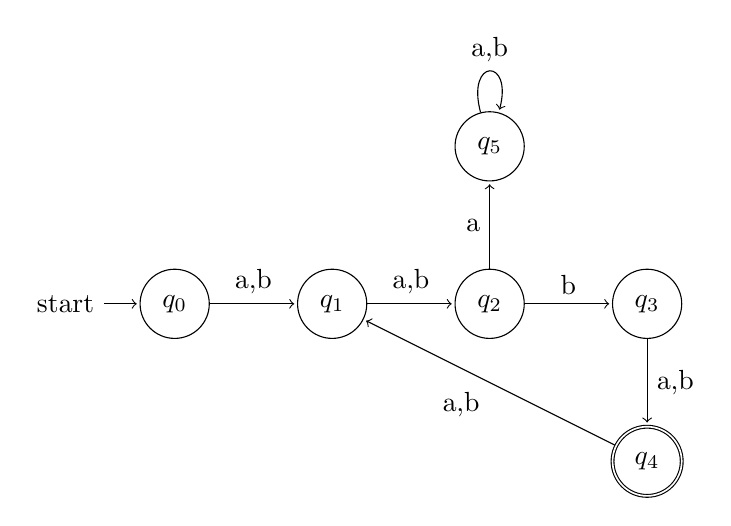
\begin{tikzpicture}[shorten >=1pt,node distance=2cm,on grid,auto]
\node[state ,initial] (q_0) {$q_0$};
\node[state] (q_1) [right=of q_0] {$q_1$}; 
\node[state] (q_2) [right=of q_1] {$q_2$};
\node[state] (q_3) [right=of q_2] {$q_3$};
\node[state,accepting] (q_4) [below=of q_3] {$q_4$};
\node[state] (q_5) [above=of q_2] {$q_5$};
 \path[->]
(q_0) edge node {a,b} (q_1)
(q_1) edge node {a,b} (q_2)
(q_2) edge node {b} (q_3)
(q_3) edge node {a,b} (q_4)
(q_4) edge node {a,b} (q_1)
(q_2) edge node {a} (q_5)
(q_5) edge [loop above] node {a,b} ();
\end{tikzpicture}
\newpage
c) \\
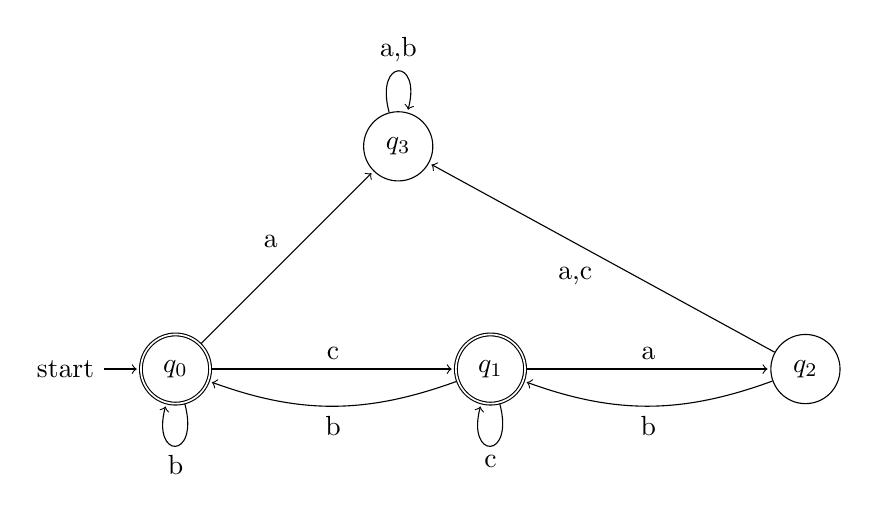
\begin{tikzpicture}[shorten >=1pt,node distance=4cm,on grid,auto]
\node[state ,initial,accepting] (q_0) {$q_0$};
\node[state,accepting] (q_1) [right=of q_0] {$q_1$}; 
\node[state] (q_2) [right=of q_1] {$q_2$};
\node[state] (q_3) [above right=of q_0] {$q_3$};
 \path[->]
(q_0) edge node {c} (q_1)
(q_0) edge [loop below] node {b} ()
(q_1) edge node {a} (q_2)
(q_1) edge [bend left=20] node {b} (q_0)
(q_0) edge node {a} (q_3)
(q_2) edge node {a,c} (q_3)
(q_2) edge [bend left=20] node {b} (q_1)
(q_1) edge [loop below] node {c} ()
(q_3) edge [loop above] node {a,b} ();
\end{tikzpicture}

\section*{Answer 3}


\subsection*{a.}
$w_{1}$ doesn't belong to the language that NFA represents. \\
\subsection*{b.}
$w_{2}$ is in the language. One of the possible configuration is as follows: \\
$(q_{0} , ababa) \vdash (q_{1} , baba) \vdash (q_{3} , baba) \vdash (q_{3} , aba) \vdash (q_{5} , ba) \vdash (q_{1} , ba) \vdash (q_{3} , ba) \vdash (q_{3} , a) \vdash (q_{5} , e)$ \\



\section*{Answer 4}

\subsection*{a.}

$bab^{*} \cup [b(a \cup b)^{*} (e \cup bab^{*} )] \cup [bab^{*} (b \cup ab) (a \cup b)^{*} (e \cup bab^{*})] $ \\

\subsection*{b.}

NFA with new initial and final state: \\
\begin{tikzpicture}[shorten >=1pt,node distance=4cm,on grid,auto]
\node[state ,initial] (q_s) {$q_s$};
\node[state] (q_0) [right=of q_s] {$q_0$};
\node[state] (q_1) [above right=of q_0] {$q_1$}; 
\node[state] (q_2) [below=of q_1] {$q_2$};
\node[state] (q_3) [below right=of q_1] {$q_3$};
\node[state,accepting] (q_f) [below right=of q_2] {$q_f$};
 \path[->]
(q_0) edge node {b} (q_1)
(q_1) edge node {a} (q_2)
(q_2) edge [bend left=20] node {b} (q_1)
(q_1) edge  node {e} (q_3)
(q_3) edge [bend left=20] node {b} (q_1)
(q_3) edge [loop above] node {a} ()
(q_2) edge [loop below] node {b} ()
(q_2) edge node {a} (q_0)
(q_2) edge node {b} (q_3)
(q_s) edge node {e} (q_0)
(q_2) edge node {e} (q_f)
(q_3) edge node {e} (q_f);
\end{tikzpicture}

q0 eliminated: \\
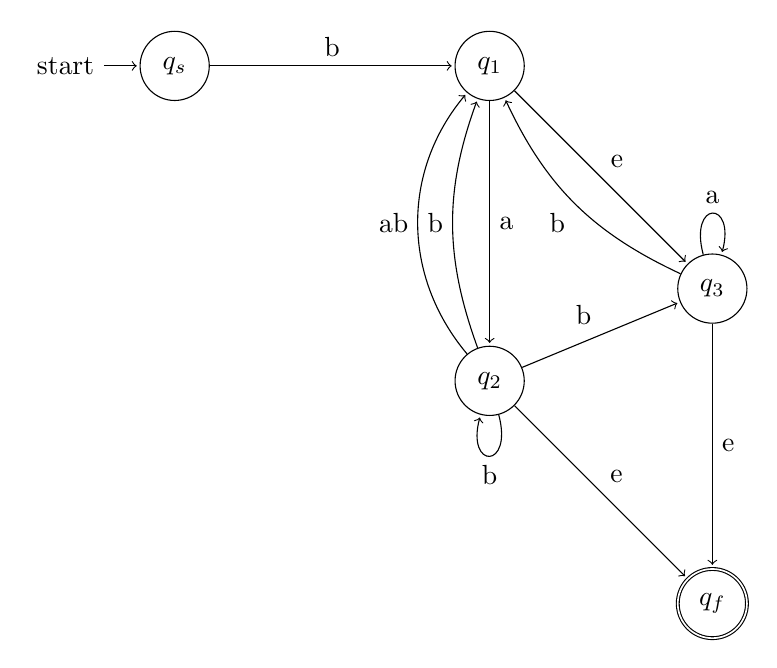
\begin{tikzpicture}[shorten >=1pt,node distance=4cm,on grid,auto]
\node[state ,initial] (q_s) {$q_s$};
\node[state] (q_1) [right=of q_s] {$q_1$}; 
\node[state] (q_2) [below=of q_1] {$q_2$};
\node[state] (q_3) [below right=of q_1] {$q_3$};
\node[state,accepting] (q_f) [below right=of q_2] {$q_f$};
 \path[->]
(q_1) edge  node {e} (q_3)
(q_3) edge [bend left=20] node {b} (q_1)
(q_3) edge [loop above] node {a} ()
(q_2) edge [loop below] node {b} ()
(q_2) edge node {b} (q_3)
(q_s) edge node {b} (q_1)
(q_2) edge node {e} (q_f)
(q_3) edge node {e} (q_f)
(q_1) edge node {a} (q_2)
(q_2) edge [bend left=20] node {b} (q_1)
(q_2) edge [bend left=40] node {ab} (q_1);
\end{tikzpicture}

\newpage

q1 eliminated: \\
\begin{tikzpicture}[shorten >=1pt,node distance=4cm,on grid,auto]
\node[state ,initial] (q_s) {$q_s$};
\node[state] (q_2) [below=of q_3] {$q_2$};
\node[state] (q_3) [above right=of q_1] {$q_3$};
\node[state,accepting] (q_f) [below right=of q_3] {$q_f$};
 \path[->]
(q_3) edge [loop above] node {a,b} ()
(q_2) edge [loop below] node {b} ()
(q_2) edge [bend left=20] node {b} (q_3)
(q_2) edge node {ab} (q_3)
(q_s) edge node {b} (q_3)
(q_s) edge node {ba} (q_2)
(q_3) edge [bend left=20] node {ba} (q_2)
(q_3) edge node {e} (q_f)
(q_2) edge [bend right=20] node {e} (q_f);
\end{tikzpicture}

q2 eliminated: \\
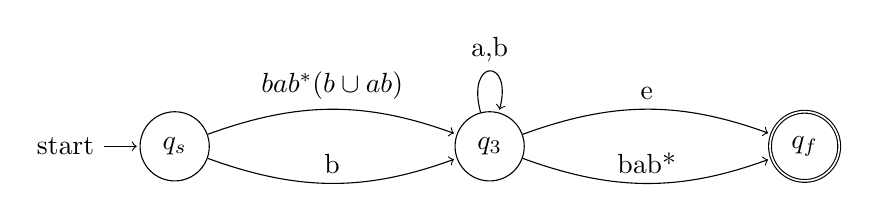
\begin{tikzpicture}[shorten >=1pt,node distance=4cm,on grid,auto]
\node[state ,initial] (q_s) {$q_s$};
\node[state] (q_3) [right=of q_s] {$q_3$};
\node[state,accepting] (q_f) [right=of q_3] {$q_f$};
 \path[->]
(q_3) edge [loop above] node {a,b} ()
(q_s) edge [bend right=20] node {b} (q_3)
(q_s) edge [bend left=20] node {$bab^{*} (b \cup ab)$} (q_3)
(q_3) edge [bend left=20] node {e} (q_f)
(q_3) edge [bend right=20] node {bab*} (q_f);
\end{tikzpicture}

q3 eliminated: \\
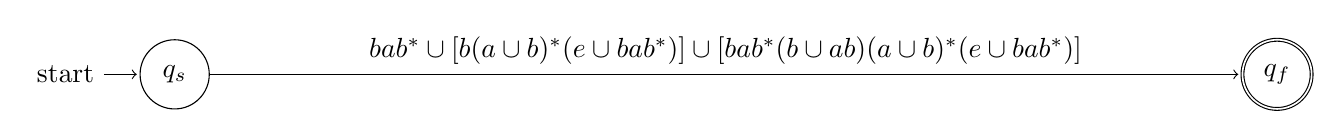
\begin{tikzpicture}[shorten >=1pt,node distance=14cm,on grid,auto]
\node[state ,initial] (q_s) {$q_s$};
\node[state,accepting] (q_f) [right=of q_s] {$q_f$};
 \path[->]
(q_s) edge node {$bab^{*} \cup [b(a \cup b)^{*} (e \cup bab^{*} )] \cup [bab^{*} (b \cup ab) (a \cup b)^{*} (e \cup bab^{*})] $} (q_f);
\end{tikzpicture}


\section*{Answer 5}
a) \\
\begin{tikzpicture}[shorten >=1pt,node distance=4cm,on grid,auto]
\node[state ,initial] (q_{00}) {$q_{00}$};
\node[state] (q_{01}) [right=of q_{00}] {$q_{01}$};
\node[state] (q_{02}) [above=of q_{01}] {$q_{02}$};
\node[state] (q_{03}) [below=of q_{01}] {$q_{03}$};
\node[state,accepting] (q_{04}) [right=of q_{01}] {$q_{04}$};
\path[->]
(q_{00}) edge node {a} (q_{02})
(q_{00}) edge node {b} (q_{03})
(q_{03}) edge [bend left=30] node {a} (q_{02})
(q_{02}) edge node {b} (q_{01})
(q_{02}) edge node {a} (q_{04})
(q_{01}) edge node {a,b} (q_{04})
(q_{03}) edge node {b} (q_{04})
(q_{04}) edge [loop right] node {a,b} ();
\end{tikzpicture}
\newline

$q_{00}$ is the set that includes $q_0$ , $q_1$ , $q_2$. \\
$q_{01}$ is the set that includes $q_1$ . \\
$q_{02}$ is the set that includes $q_1$ , $q_3$. \\
$q_{03}$ is the set that includes $q_2$. \\
$q_{04}$ is the empty set. \\

b) \\

\section*{Answer 6}

We know that regular languages are closed under intersection and complementation. Because $L1 - L2 = L1 \cap  \overline{L2}$ and 
every NFA has an equivalent DFA , regular languages are closed under set difference. \\ 

\section*{Answer 7}

\subsection*{a.}
Let's choose the pumping length as $\frac{ p^2 }{2}$ and get a string of length $p^2$ which is $a^{ p^2 } = s$ from the language and assume that L is a regular language. Then, it must satisfy the pumping lemma. \\
Make $s=xyz$ , $x=a^{ p^2 }$ and $y=a^{p^2}$. Then, $xy^{i}z$ becomes $a^{ \frac{ p^2 (i+2)}{2 } }$. \\
This $xy^{i}z$ must be in the language for all i. However, it only satisfies for 1,7,17... So, L is not regular. \\
\subsection*{b.}




\end{document}

​

